\section{Proposed architechture}
\label{sec:propesedArch}

\begin{figure}[t!]
\centering
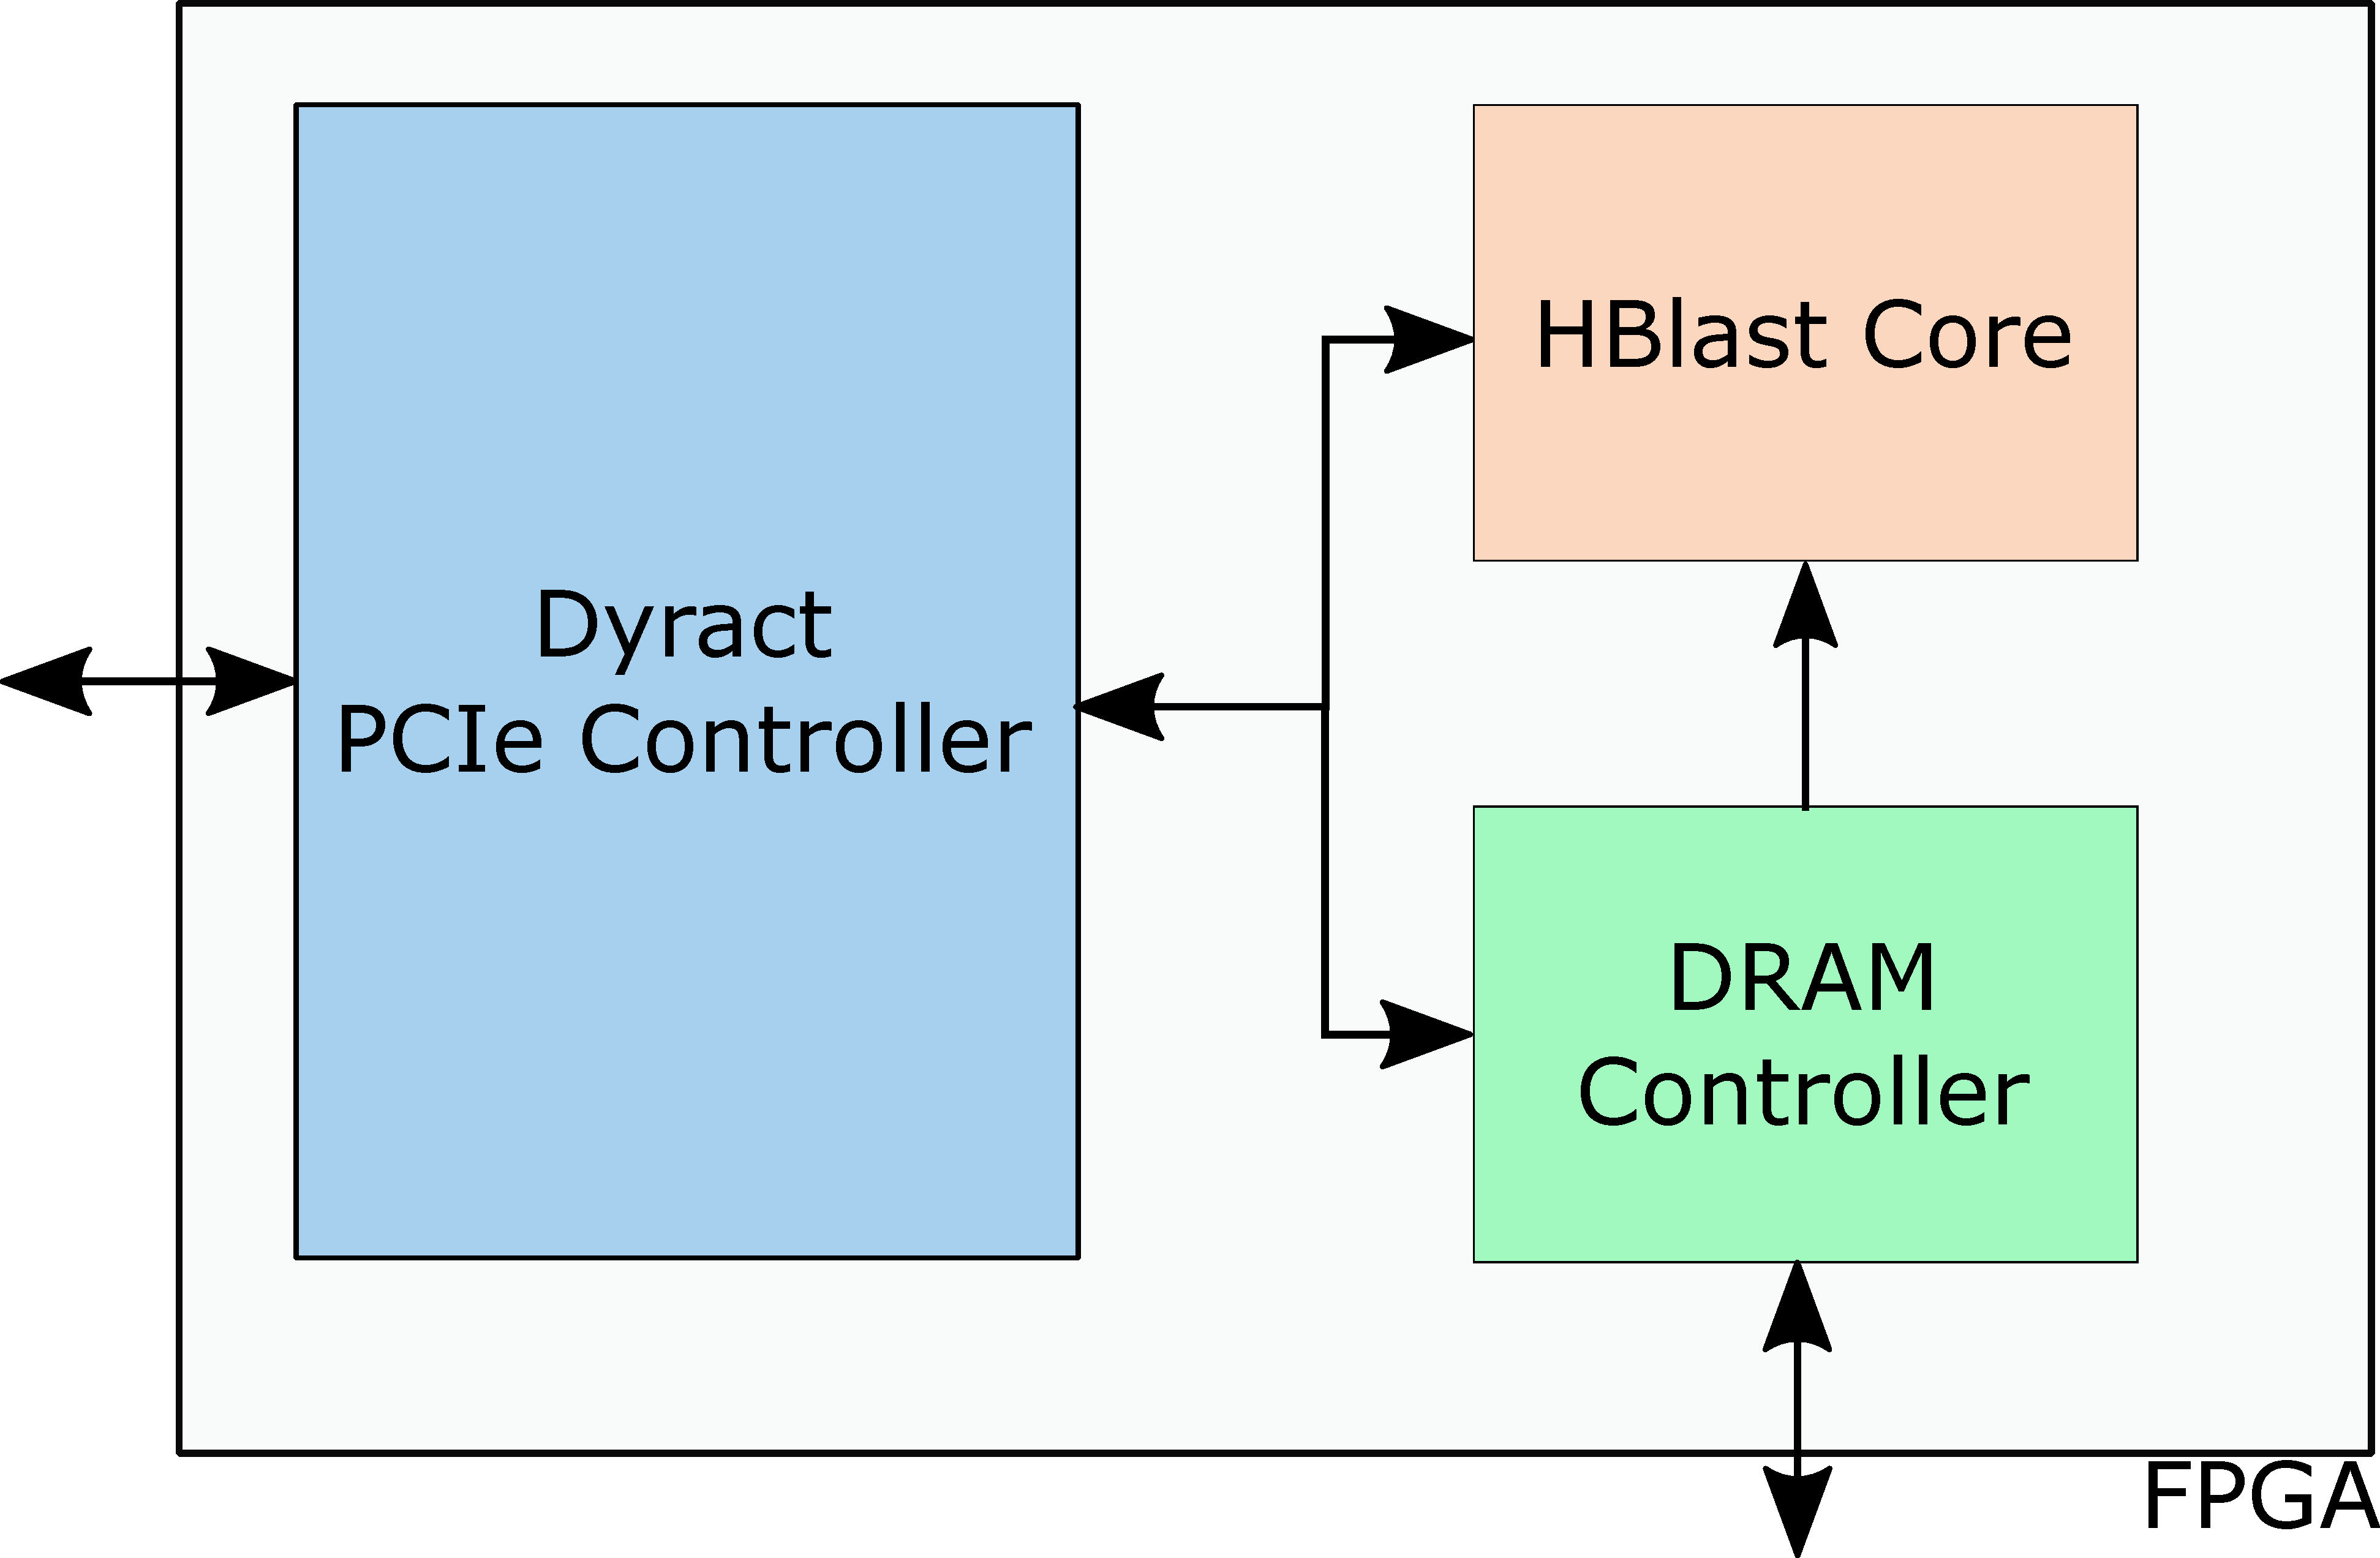
\includegraphics[width=0.9\columnwidth]{Figures/sysArch.pdf}
\caption{Overall architecture of HBlast targeting on-premise FPGA implementation} \label{fig:sysArch}
\end{figure}

The overall architecture of HBlast library targeting on-premises implementation is as depicted in Fig.~\ref{fig:sysArch}.
It is implemented on an off-the-shelf vendor supported FPGA development board (Xilinx~VC709).
This board supports a PCIe x8 Gen.3 interface which theoretically supports up to 7.88 GB/s/direction bandwidth.
It has 8GB external DRAM, supporting up to 933MHz clock frequency.
The implementation consists of an IP core (Dyract) to interface with a host computer, a DRAM controller for interfacing with the external DDR memory and the module implementing the core BLAST algorithm.
Details of each sub-module is discussed in the subsequent sections.

Our current implementation targets only DNA sequence searching which could be augmented with support for protein searching in the future.
Since there are only 4 types of nucleobases encountered in DNA sequences (adenine (A), guanine (G) cytosine (C), and thymine (T)), only two bits are used to represent each base.
This considerably reduces the memory requirement for storing the database compared to traditional character-based storage since each character takes one byte of data.
The entire database is initially stored in the external DRAM memory of the FPGA-board and the query sequences are stored in the FPGA internal memory.

\subsection{PCIe Controller}
We use our previously developed open-source FPGA PCIe controller called Dyract to interface with the host computer~\cite{Vipin2014}.
The PCIe interface is used to send the database and query strings to the FPGA as well as to receive back the HSPs and the corresponding scores.
This interface can provide up to 6.5 GB/s throughput, nearly saturating the available PCIe bandwidth.
The PCIe controller is interfaced with both the memory controller as well as the BLast core.
Depending upon the stream type, data is sent either to the external DRAM or the internal registers of BLast core through a bridge logic.

%Since the database needs to be stored only once in the external DRAM, the PCIe bandwidth is not critical to the overall performance of the system. Hence for systems which do not support PCIe, this interface could be replaced with low-bandwidth interfaces such as Ethernet or even serial.

\subsection{DRAM Controller}
The DRAM controller internally uses Xilinx memory interface generator (MIG) IP core~\cite{mig2018}. 
Present implementation instantiates a single MIG controller thus supporting up to 4GB external memory on VC709.
The interface operates at 200MHz with 512-bit interface providing a maximum of 12.5 GB/s throughput.
The throughput of the memory interface is very critical to the overall performance since the database sequences are continuously read from the external memory for comparing with the query sequence.
Multiple levels of pipelining is implemented to support the required memory clock performance.

\subsection{BHlast Core}

\begin{figure}[t!]
\centering
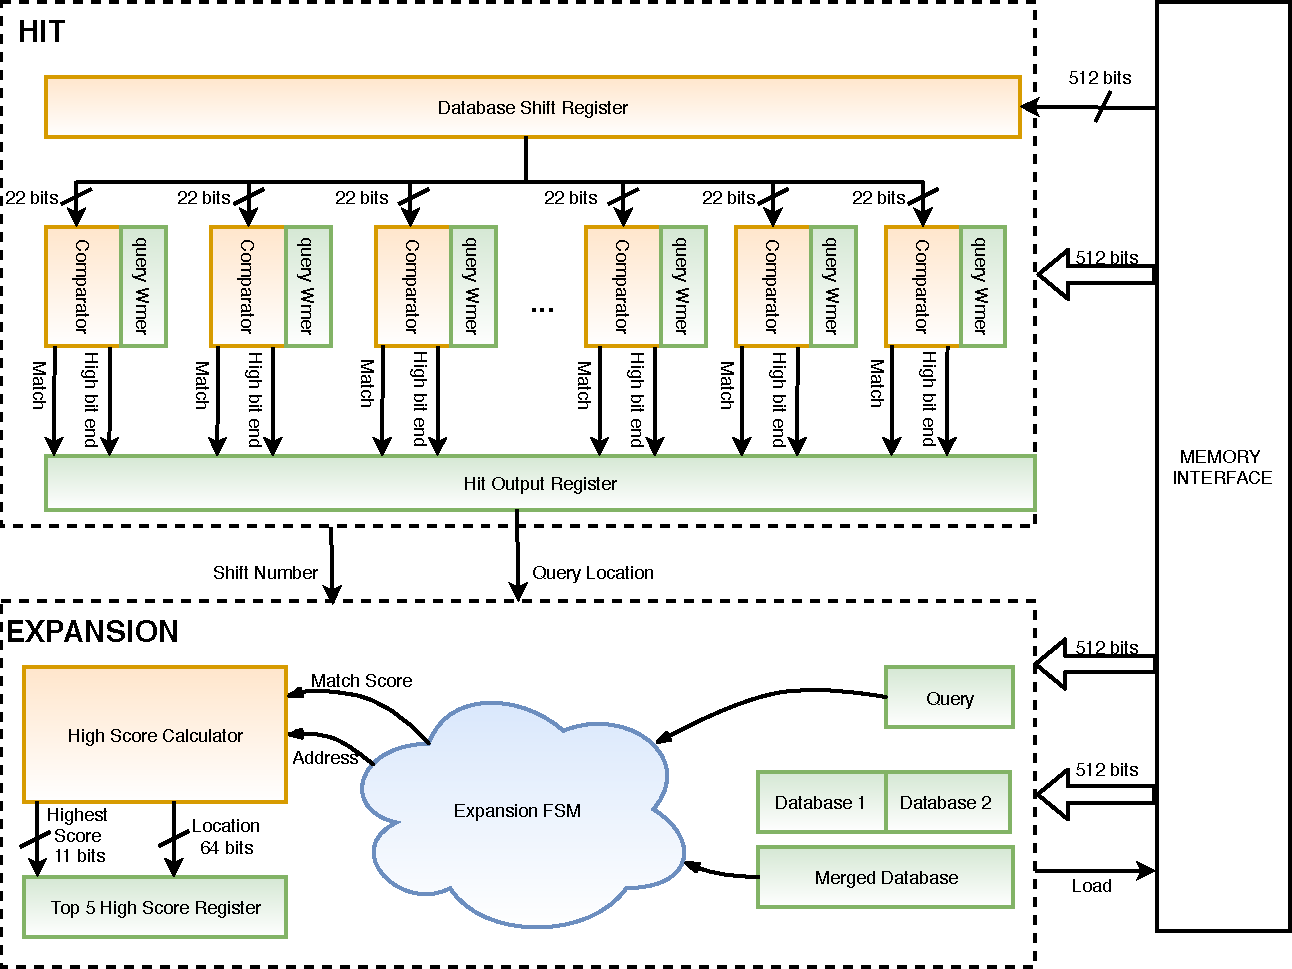
\includegraphics[width=\columnwidth]{Figures/BlastMachine.pdf}
\caption{Detailed architecture of the HBlast core module showing the Hit and Expansion submodule and their interconnection} \label{fig:blastArch}
\end{figure}

This module implements the core BLAST algorithm discussed in Section~\ref{sec:blast}.
For the current implementation, the maximum query size supported is 512bits~(256 bases) with up to 4GB database. 
This can be extended to larger size by instantiating more number of basic compute units.
The database is stored in the external DRAM memory and the query sequence is stored in the internal \textit{queryReg} register.
The two main sub-modules of the HBlast core are the \textit{Hit} and \textit{Expansion} modules as shown in Fig.~\ref{fig:blastArch}. As their names state, these blocks are responsible for tasks like finding hit (match), expanding the sequence and linking blocks. 

For the nucleotides, W-mer size is 11 letters~\cite{kasap2008design}, so by \textit{Eq.\ref{eq1}} there are 246 W-mers in 256-letter query. 
Each of them must be compared with each W-mer of the database.  
Comparison between one database and one query W-mer at a time is not effective in terms of latency. 
In HBlast architecture this operation is parallelized by introducing 246 comparators (one for each query W-mer). 
All comparators have common 22-bit (11-letter) database W-mer fetched from external memory. 
This input is controlled by the \textit{Database Shift Register}, which performs a 2-bit shift operation after every clock cycle. 
The expansion module will be activated if output of any of these comparators is high, indicating a valid match has been found between the database and the query. 

The expansion and hit are sequential operations, meaning the expansion will start only if the hit stops and other way around. 
A single expansion block is used to restrict the FPGA resource utilization and thus to improve the clock performance.
Once a valid match is found, the hit module sends information regarding the location of the match in the query and the number of performed shift operations to the expand module. 
  
\subsection{Hit}
The hit module compares W-mers from the database with W-mers in query in parallel to find exact matches. 
The module implements a finite state machine (FSM) with two states as shown in Fig.\ref{fig:hitFSM}. 
In the Idle state, the module takes a 22-bit sequence from the database and compares each W-mer with the corresponding W-mers in the query sequence via 246 comparators. 
Due to the parallel architecture, the comparisons happen simultaneously which significantly improves the latency. 
If at least one exact match is detected, the signal \textit{hit} is activated and the process passes to the next state, (\textit{HitLow}).
It stays in this state while expansion process is being performed. When expansion is over, the FSM goes back to the \textit{Idle state} and verifies if there are other matches of the W-mers within the query. 
If there is a match again, the expansion process will be repeated, if there is no more match found, the loaded 512 bits of database is shifted by 2 bits and next 22 bits of sequence in database are compared with the query. 
When all W-mers in the database are compared, the next 512 bits of the database are loaded from the external memory and process is repeated. 

\begin{figure}[t!]
\centering
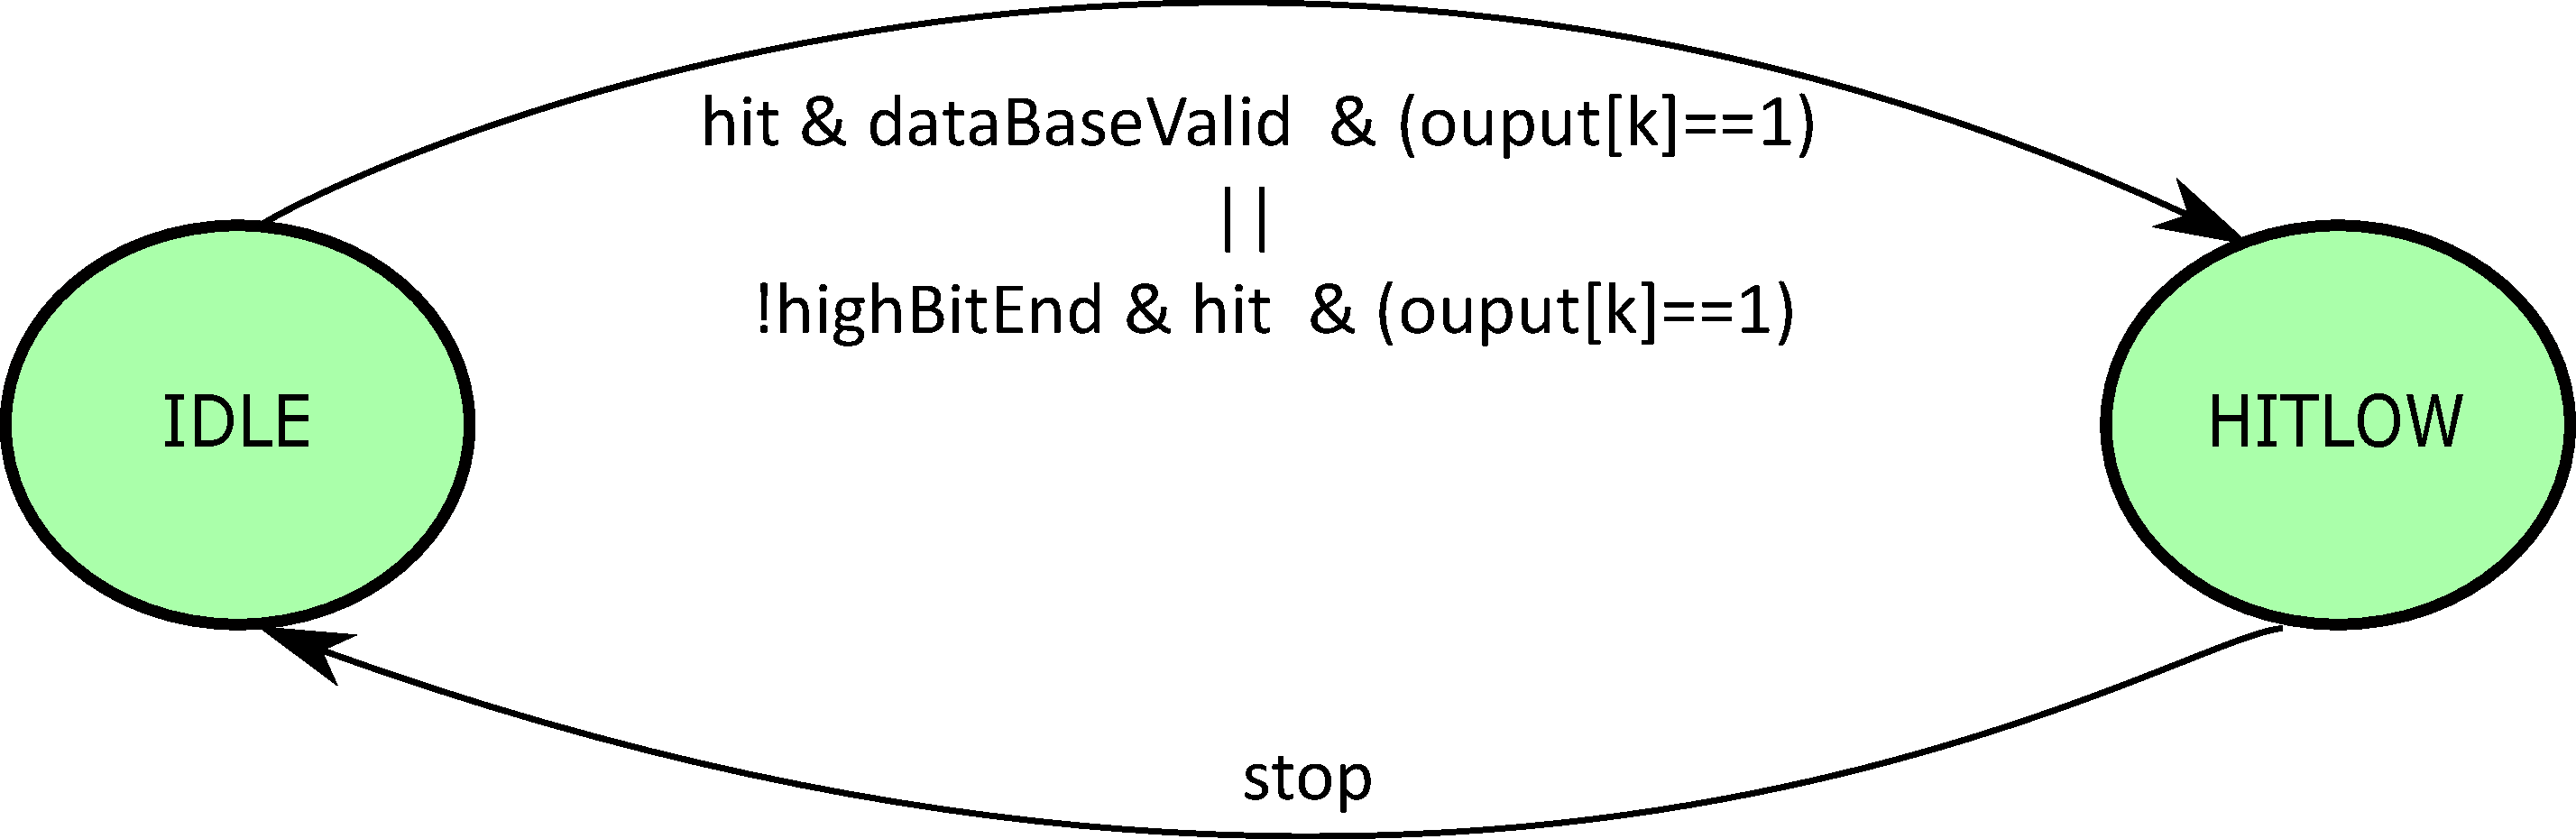
\includegraphics[width=0.7\columnwidth]{Figures/hitFSM.pdf}
\caption{FSM diagram for module Hit} \label{fig:hitFSM}
\end{figure}



\subsection{Expansion}
The Expansion Finite State Machine expands the exactly matched sequences of the database to both sides by comparing it with the query. 
The outputs from this module are the start and end locations of the most matching five expanded sequences and their high scores. The FSM consists of 6 states as shown in Fig.~\ref{fig:expandFSM}.

\begin{enumerate}
  \item \textbf{Idle}: The FSM stays in this state until it receives the \textit{start} signal signal from the \textit{hit} module.
  \item \textbf{Wait}: In this state module waits until it receives the database portion from the external DRAM.
  \item \textbf{Load 1}: This state loads the 512-bits of database to a register. Then it passes to the next state according to the shift number by following logic: if the shift number is less than 199 or more than 290, it goes to state \textbf{Load 2}; otherwise it goes to the \textbf{Expand} state directly. 
  \item \textbf{Load 2}: This state takes another 512-bit piece of database located either before or after the database with exact matched sequence. This is to satisfy the boundary condition, where an exact match is detected at the boundary of the current database sequence stored in the FPGA. In order to expand, the next piece of database has to be fetched from the external memory. 
The starting address of the next sequence is calculated within the state and it goes to the next state which waits for data from the DRAM. 
  \item \textbf{Merge}: In this state the 512-bit sequence of the database is merged with the next 512-bit sequence to satisfy the boundary conditions.
  \item \textbf{Expand}: The exactly matched W-mers of database and query expands to both sides by 2 bits each clock.
\end{enumerate}

The initial score of HSP is 55 (obtained from 11*5). 
If next 2 bits are matched 5 is added to the HSP score, otherwise 4 points are deducted. 
Threshold value is chosen to be 200 bits, meaning that the sequence can be expanded to both sides by 200 bits each. 
Accordingly, maximum HSP can be 1055. 
The threshold value is set to 200 since the maximum query sequence size is 512-bits.
The expansion is performed with all the matching W-mers of the query with the database. And as the final output the 5 sequences with the highest score, that is 5 most matching sequences of the query to database, is obtained with their positions as start and end locations in the database. However, the operation stops when the exact matching sequence with highest score of 1055 is detected.
There is no need of further matches since the that is the maximum possible score for an HSP.
       

\begin{figure}[t!]
\centering
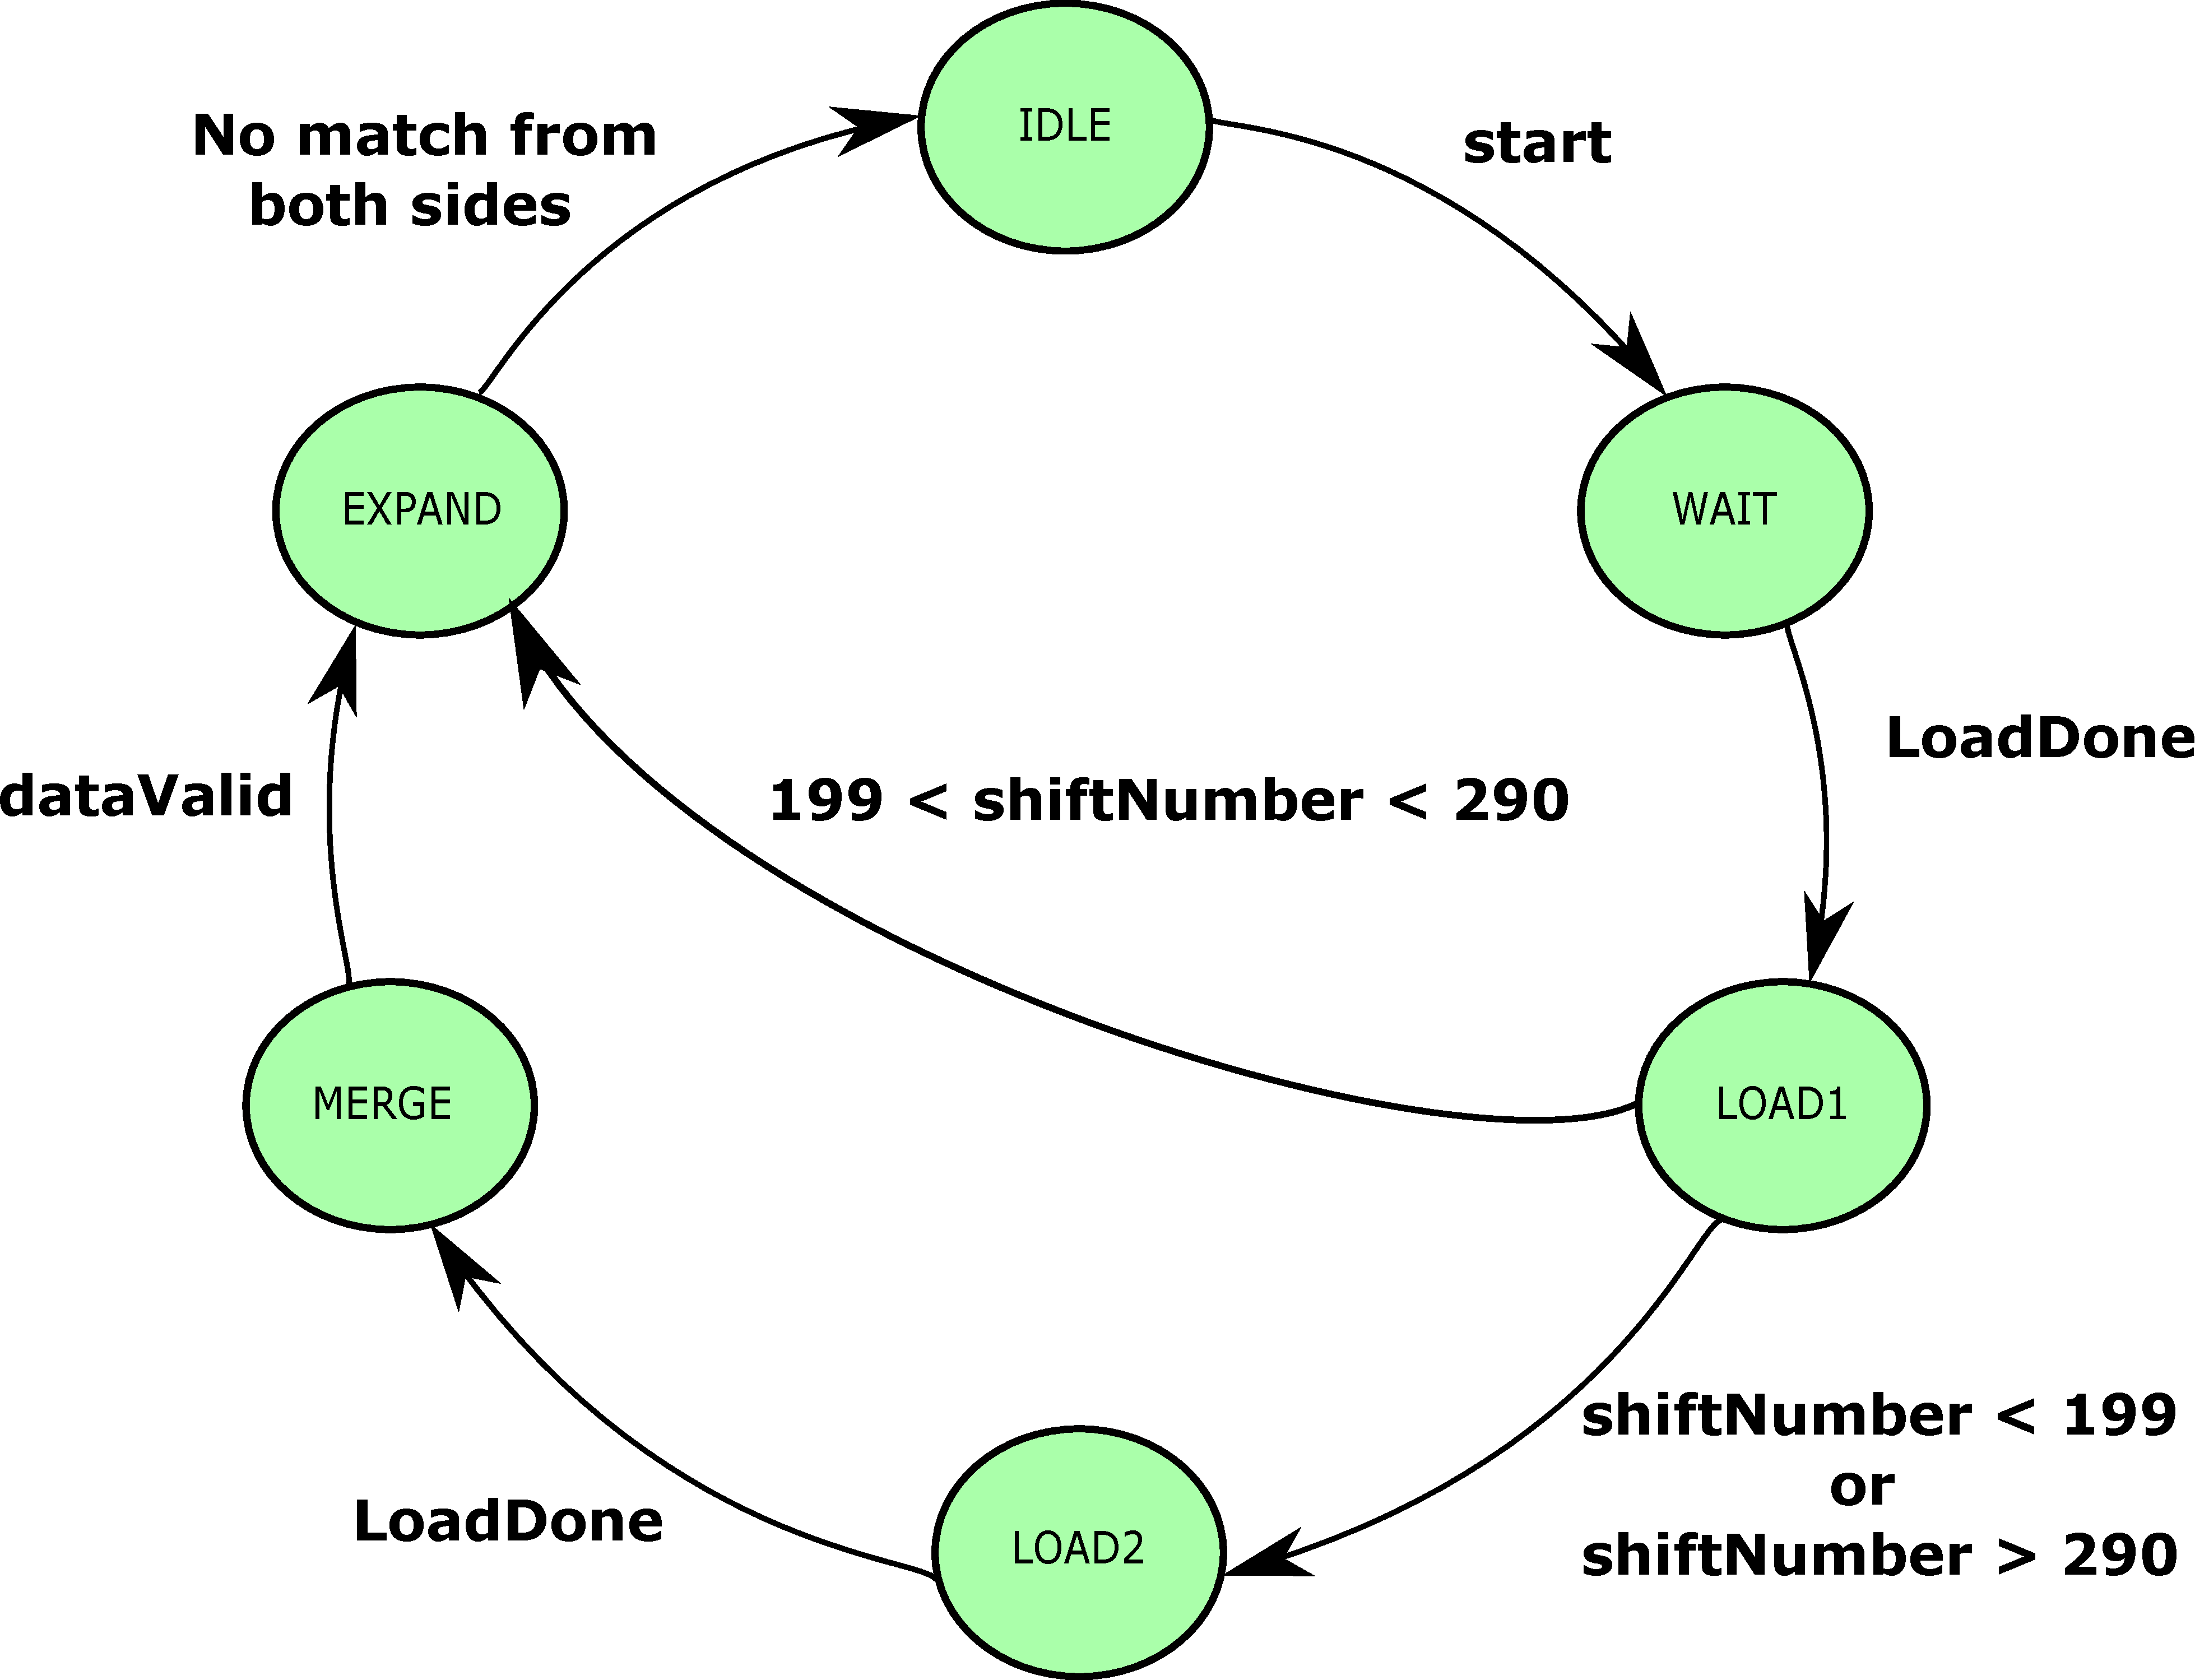
\includegraphics[width=\columnwidth]{Figures/expandFSM.pdf}
\caption{FSM diagram for module Expansion} \label{fig:expandFSM}
\end{figure}
       
       
\subsection{Memory Interface}
The module Memory Interface is a control unit that interacts with modules Expansion FSM, Hit and bridge. 
It is an FSM of 7 states. The main functions of the module are following:
\begin{itemize}
\item The module takes addresses from the expansion or hit modules and sends the control signals to the DRAM controller.
\item When it gets signal which indicates the absence or expiration in matches between query and 22-bit W-mer of the database from Hit module, it sends signal to shift the current piece of the database to the module.
\item The module arbitrates the memory access between the Expansion and Hit modules. 
\end{itemize}

%\begin{figure}
%\centering
%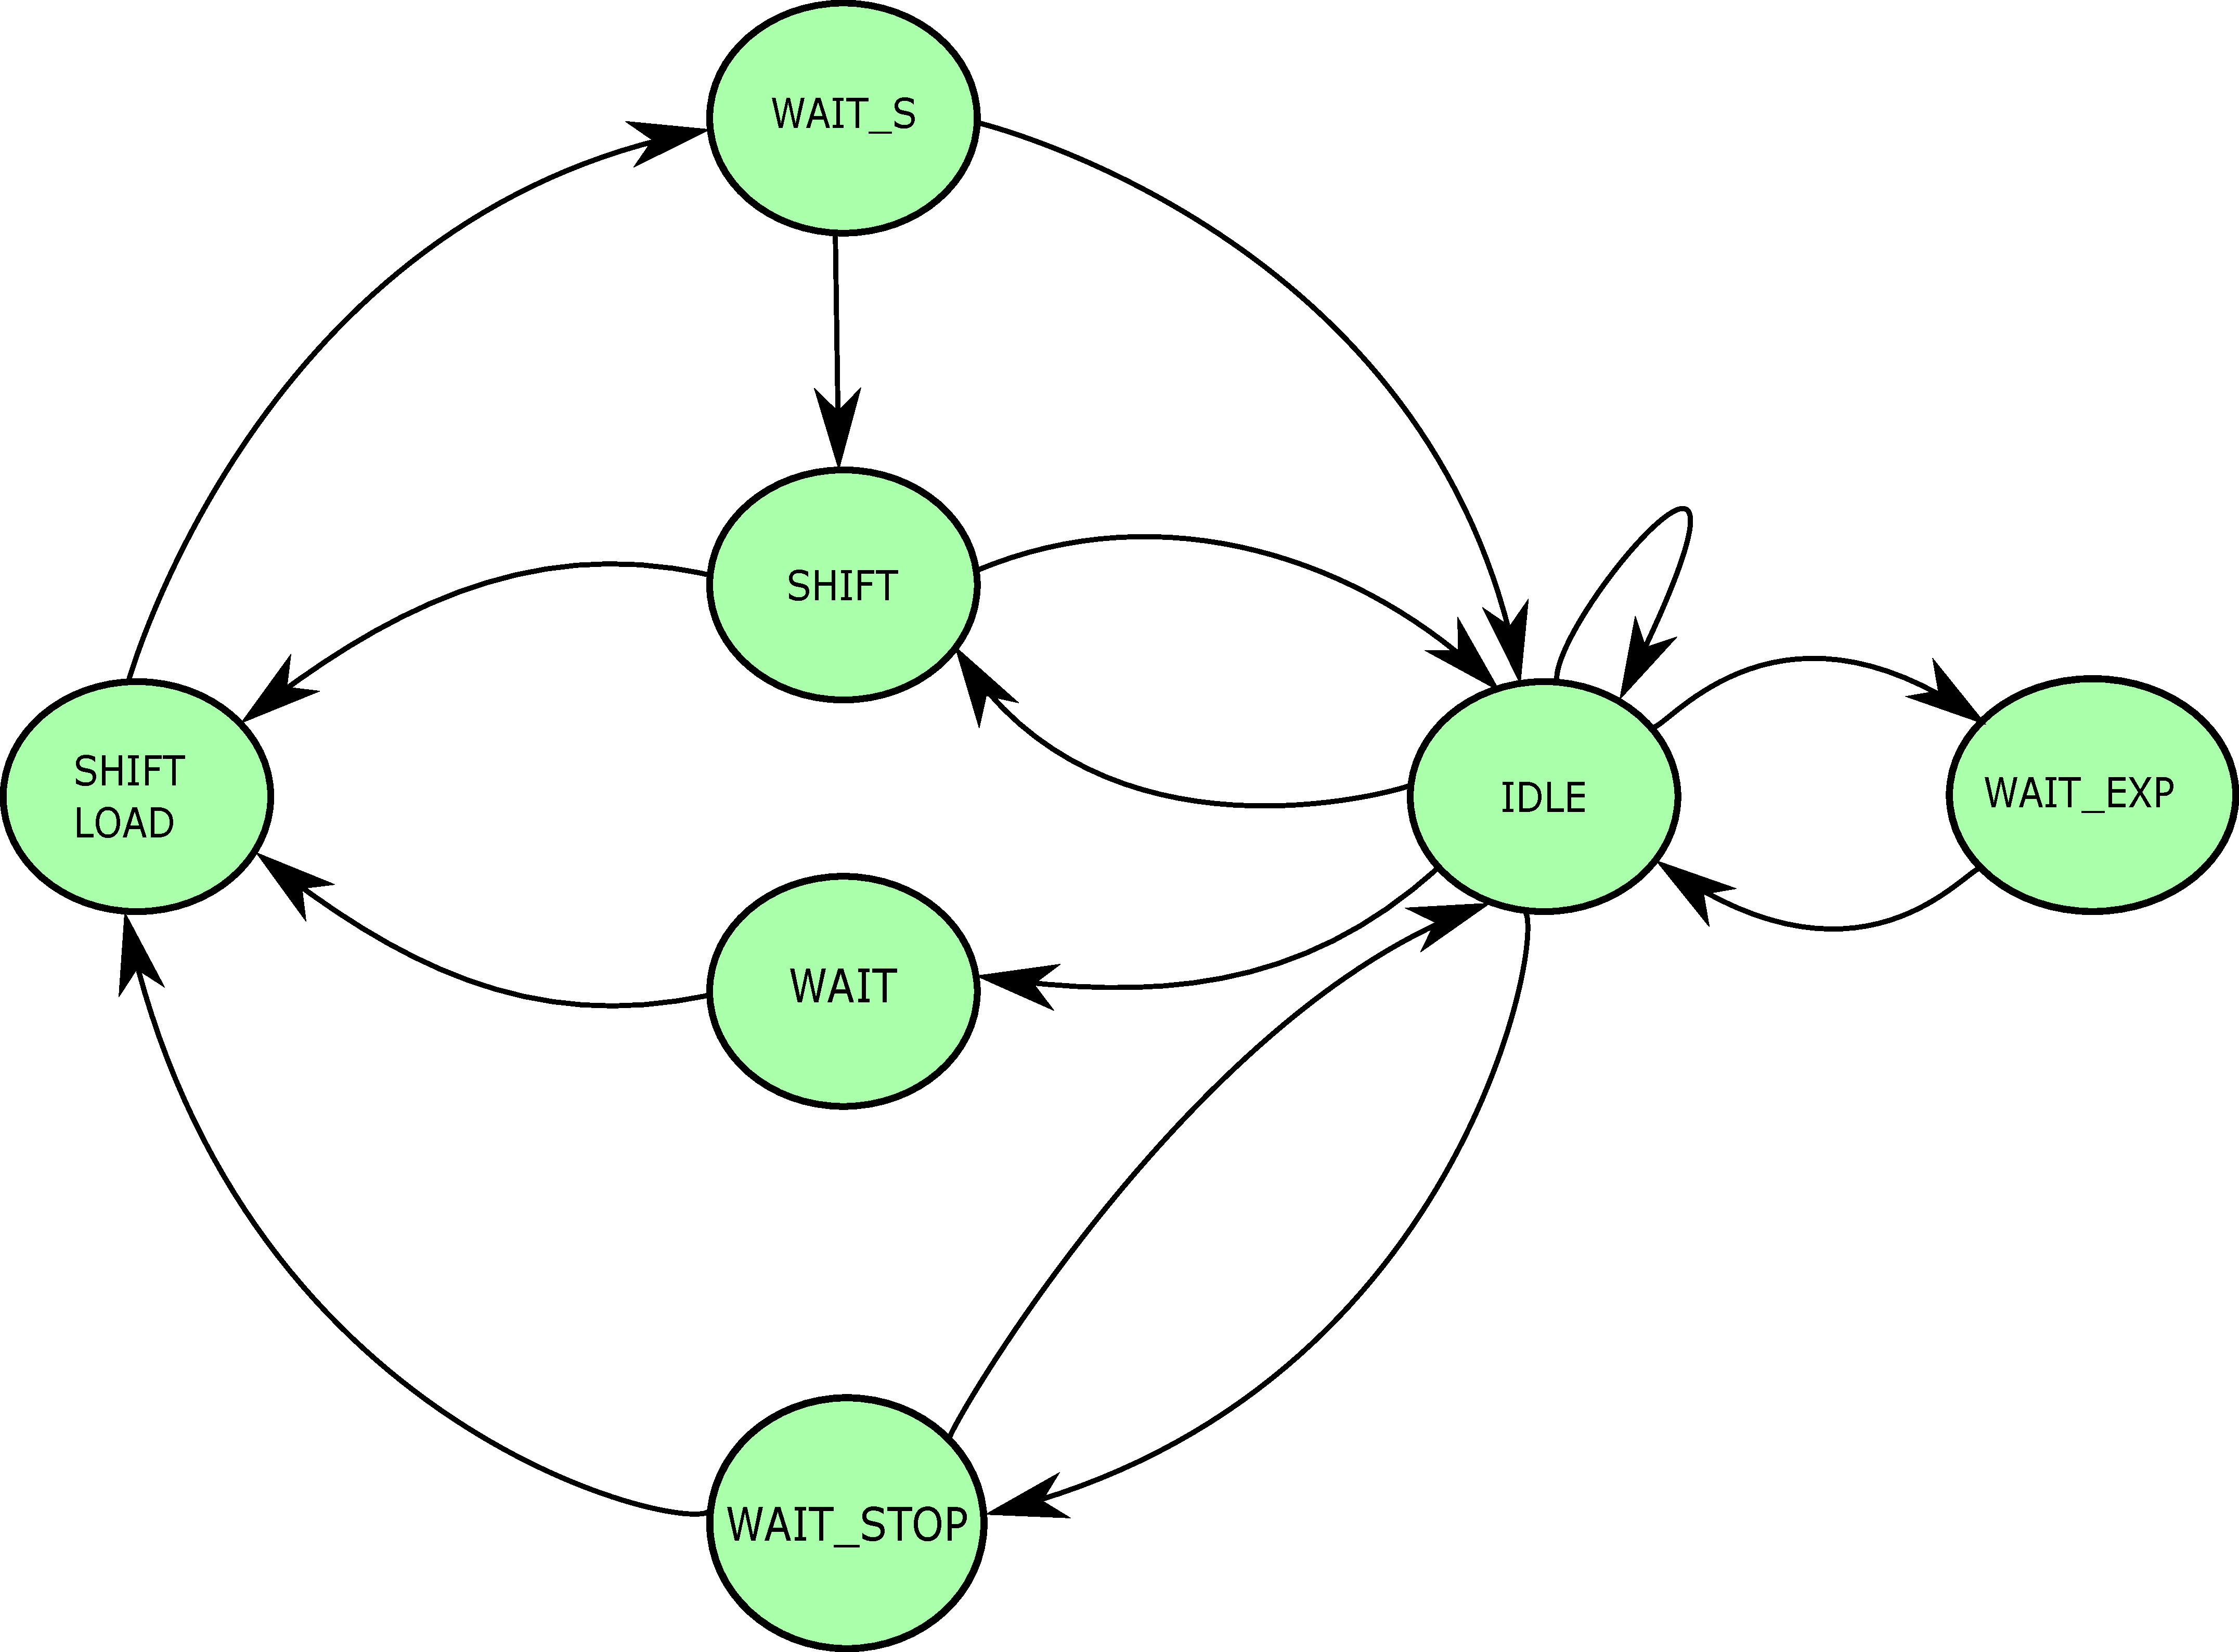
\includegraphics[width=\columnwidth]{Figures/FSM_Mem_New.pdf}
%\caption{FSM diagram for Memory Interface} \label{fig:MemInt}
%\end{figure}


\subsection{Bridge}
The Bridge module implements the data width matching between the PCIe interface and the Memory Interface and arbitrates the memory access between the PCIe core and the BLast core. 
It consists of four states, refer to Fig.~\ref{fig:bridge}:
\begin{enumerate}
\item \textbf{Idle}. Depending on whether input signal is write or read, the state changes to Wait\_wr\_cmd and Wait\_rd respectively. 
Write signal comes from PCIe when it wants to write query data and database into DRAM. 
While, read signal comes from two main modules (Hit and Expand) of the architecture when it wants to take data from DDR.
\item \textbf{Wait\_wr\_cmd}. This state waits for the acknowledgement from DDR, as it is received, input data is sent to DDR. Then, state changes to the next Wait\_wr state.
\item \textbf{Wait\_wr}. The FSM state waits for write\_ready acknowledgment, and then increments the write address by 8.
The DRAM interface from FPGA is 64-bit wide hence to write 512-bit sequence, 8 write operations are required. 
\item \textbf{Wait\_rd}. After receiving read ready signal from DRAM controller, it reads data 8 times and each time increments address by 8 for the same reason as explained above. 
\end{enumerate}


\begin{figure}
\centering
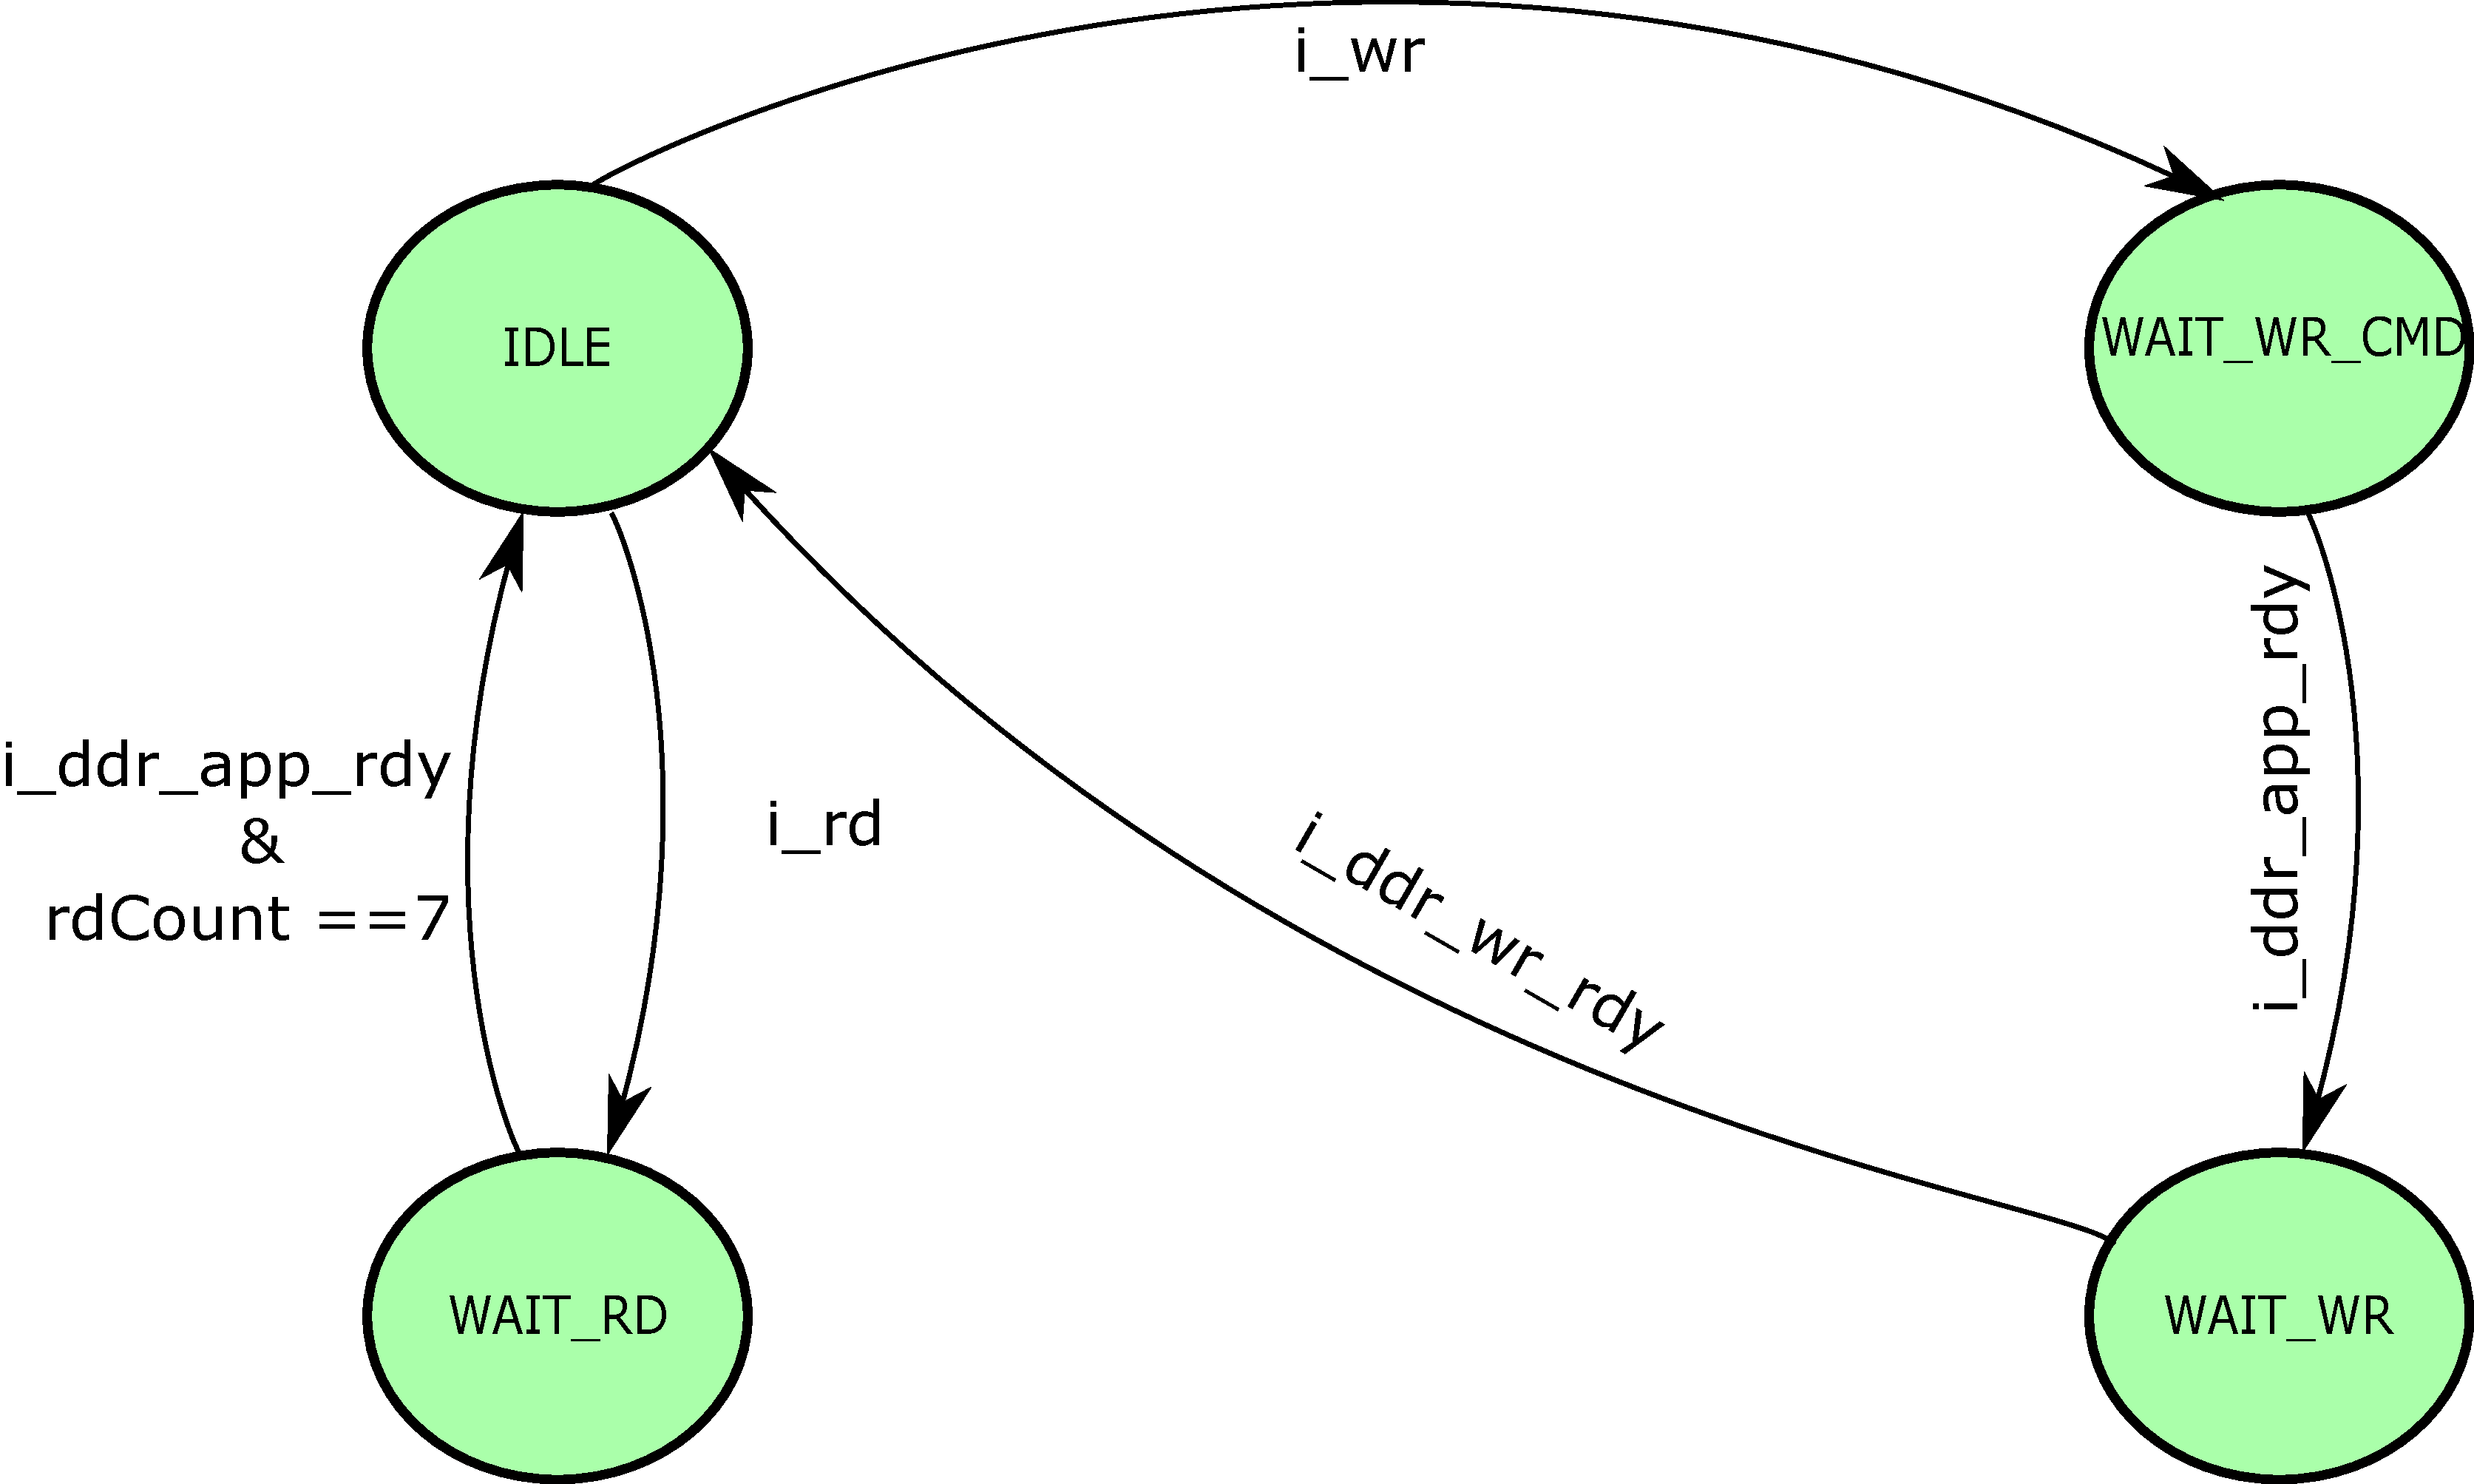
\includegraphics[width=\columnwidth]{Figures/bridgeFSM.pdf}
\caption{FSM diagram for bridge} \label{fig:bridge}
\end{figure}

\subsection{HBlast Cloud Architecture}
Fig.~\ref{fig:awsArch} depicts the architecture of the HBlast module when implemented on an AWS-EC2 F1 FPGA instance~\cite{aws2018}.
The F1 instance is a Xilinx Ultrascale+ FPGA and supports PCIe Gen3 x16 interface to the host computer.
Thus, it supports twice the bandwidth between the host computer and FPGA compared to VC709 implementation.
Each instance has 64GB external DRAM (DDR4) memory support also.
Amazon provides a \emph{shell} infrastructure for the FPGA, which manages the communication between the FPGA and the host machine as well as between the FPGA and the external DRAM memory.
This eliminates the need for the Dyract IP and the DRAM controller when targeting the design for the cloud infrastructure.


\begin{figure}[t!]
\centering
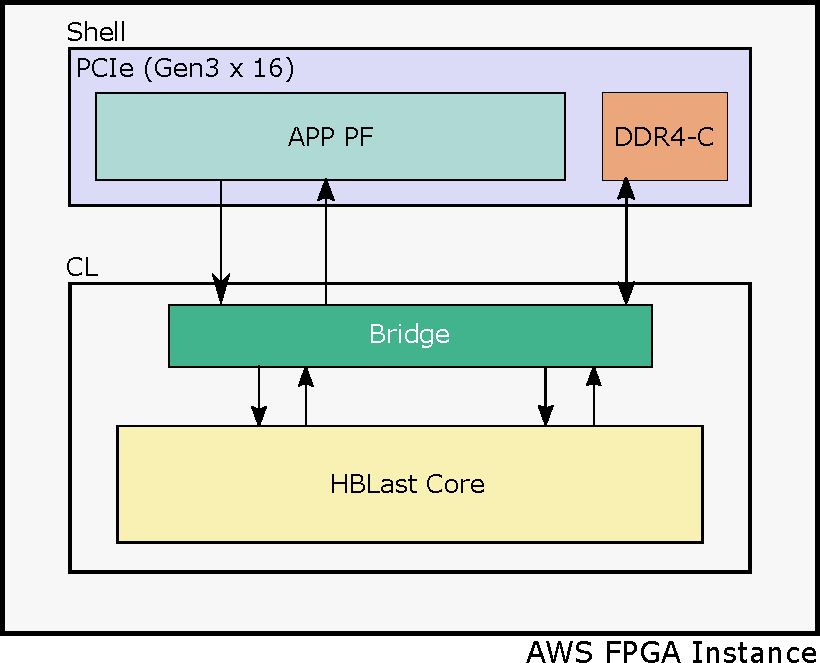
\includegraphics[width=0.9\columnwidth]{Figures/AwsArch.pdf}
\caption{HBlast architecture when targeting Amazon EC2 F1 FPGA instance} \label{fig:awsArch}
\end{figure}


The bridge logic and the HBLast core are implemented in the \emph{custom logic~(CL)} portion for the F1 instance.
The bridge logic is interfaced with PCIe master and slave interfaces of the shell as well as one of the master ports of the shell DRAM interface.
Similar to the bridge logic of the on-premise implementation, this logic routes the data coming from the host server either to the external DRAM or to the internal memory of the HBLast core depending on the data stream type (database or query).  
The HBLast module instantiates the same modules as discussed before and runs at 200MHz clock frequency provided by the shell logic.